\section{Experiment Results\label{sec:results}}

%when the available clues for alignment are sparse, we have performed comparative evaluation of our model against several baselines.


\subsection{Overall Performance\label{overall}}


\cparagraph{Results on $\bf DBP15K_{FR-EN}$} Table~\ref{cross} reports the results of all the compared approaches on $DBP15K_{FR-EN}$
dataset. We apply each approach
 to two alignment directions: French to English and vice versa. This dataset requires us to handle
cross-lingual data through rough machine translation which is likely to introduce lots of noise. We report the performance of JAPE on the
two implementations presented at
 ~\cite{sun2017cross} when using structure embedding (SE), and structure and attribute joint embedding (SE+AE).
For Hits@1, our \HRGCN (SE+AE)
outperforms all other approaches by delivering the highest score. This is due to the capability of \HRGCN
(SE+AE) in preventing noisy nodes from driving the \KG representations. For Hits@10, JAPE (SE+AE), with the help of aligned relations for training,
 gives the best performance, with an improvement of 10\%$\sim$13\% over \HRGCN (SE+AE). However, our approach has the advantage for not relying on aligned
relations and attributes, thus has lower overhead.


\cparagraph{Results on WBD} Table~\ref{f1} reports the performance of all models on WBD dataset. While the vanilla \GCN performs worse than
ITransE$'$, by adding highway gates to control the noise, \HGCN is able to outperform all existing approaches. By introducing highway gates and pre-defined node features to \RGCN, our \HRGCN (SE+AE) model delivers the best Hits@k score in both alignment directions,
improving upon ITransE$'$ by 38.9\% and 41.6\% for Hits@1 and Hits@10, respectively in the direction of
Baidu$\rightarrow$Wiki. This shows that our model has a distinct advantage in entity alignment over existing approaches.

\begin{table}
	\centering
	% \small
	\scriptsize
	\begin{tabular}{lrrrr}
		\toprule
		\multirow{2}{*}{$\bf DBP15K_{FR-EN}$} & \multicolumn{2}{c|}{$\bf FR \rightarrow EN$} & \multicolumn{2}{c}{$\bf EN \rightarrow FR$} \\
		& \bf Hits@1 & \bf Hits@10 & \bf Hits@1 & \bf Hits@10 \\
		\midrule
		\rowcolor{Gray}JE & 15.3 & 38.8 & 14.6 & 37.2 \\
		ITransE$'$ & 14.9 & 31.5 & 13.6 & 29.8 \\
		\rowcolor{Gray}MTransE & 24.4 & 55.5 & 21.2 & 50.6 \\
		JAPE (SE) & 29.6 & 64.5 & 26.5 & 60.3 \\
		\rowcolor{Gray}JAPE (SE+AE) & 32.3 & \bf 66.6 & 32.9 & \bf 65.9 \\
		\GCN & 15.3 & 32.1 & 13.6 & 31.9 \\
		\rowcolor{Gray}\HGCN & 19.6 & 36.9 & 18.4 & 35.5 \\
		\RGCN & 30.5 & 33.7 & 29.4 & 31.8 \\
		\rowcolor{Gray}\bf \HRGCN (w/o $X$) & 27.1 & 31.9 & 27.1 & 32.4 \\
		\bf \HRGCN (SE) & 33.4& 35.7& 31.2& 34.6 \\
		\rowcolor{Gray} 	\bf \HRGCN (SE+AE) & \bf 44.8 & 56.6 &\bf 41.0 & 52.9 \\
		\bottomrule
	\end{tabular}
	\caption{Performance on $DBP15K_{FR-EN}$ dataset.}
	\label{cross}
\end{table}

\begin{table}
	\centering
	% \small
	\scriptsize
	\begin{tabular}{lrrrr}
		\toprule
		\multirow{2}{*}{\bf Models} &  \multicolumn{2}{c|}{$\bf Baidu \rightarrow Wiki$} & \multicolumn{2}{c}{$\bf Wiki \rightarrow Baidu$} \\
		& \bf Hits@1 & \bf Hits@10 & \bf Hits@1 & \bf Hits@10 \\
		\midrule
		\rowcolor{Gray} JE & 14.8 & 21.6 & 13.2 & 20.3 \\
		ITransE$'$ & 19.4 & 25.5 & 17.6 & 24.8 \\
		\rowcolor{Gray} \GCN & 17.1 & 27.3 & 15.7 & 25.9 \\
		\HGCN & 19.5 & 29.6 & 19.4 & 29.5  \\
		\rowcolor{Gray} \RGCN & 37.3 & 51.5 & 34.8 & 51.6 \\
		\bf \HRGCN (w/o $X$) & 15.0 & 21.7 & 14.5 & 21.5 \\
		\rowcolor{Gray} \bf \HRGCN (SE) & 50.7 & 64.3 & 49.2 & 62.6 \\
		\bf \HRGCN (SE+AE) & \bf 58.3 & \bf 67.1 & \bf 57.8{\tiny } & \bf 65.7 \\
		\bottomrule
	\end{tabular}
	\caption{Performance on WBD dataset.}
	\label{f1}
\end{table}

\subsection{Analysis\label{sec:analysis}}


%An extra advantage of GCN is that we can stack multiple convolution layers to capture more global and larger contextual and neighboring characteristics

We now provide a detailed analysis to compare different approaches.

\cparagraph{\GCN vs. prior methods}
On WBD dataset, the vanilla \GCN model outperforms JE regarding all Hits@k and performs better than ITransE$'$ in Hits@10 for both alignment directions. on $DBP15K_{FR-EN}$ dataset, \GCN achieves better results than ITransE$'$ in both directions. As aforementioned, \GCNs leverage convolutional layers to characterize an entity through careful investigations about its neighbors, including both neighboring entities and attribute values, which can provide more accurate modeling and representation for the target entity.

\cparagraph{\GCN vs. \RGCN} As shown in both Table~\ref{f1} and Table~\ref{cross}, comparing with \GCN, \RGCN further boosts the performance on both datasets, showing that introducing highly multi-relational information to the \GCN framework can achieve significant improvements on KG representations.


\cparagraph{(SE+AE) vs. (SE)}
Comparing the results of \HRGCN (SE+AE) and \HRGCN (SE) on both datasets, we can see that adding attribute embedding greatly improves the performance, resulting in a 11.39\% jump in Hits@1 and 20.96\% in Hits@10 in the direction of FR$\rightarrow$EN in Table~\ref{cross}, showing again the importance of attribute information for entity alignment.
When comparing our full model \HRGCN with \HRGCN (w/o $X$) in Table~\ref{cross} and in Table~\ref{f1}, we find that removing semantic/attribute information $X$ from node representations leads to drops of more than 20\% on $DBP15K_{FR-EN}$ dataset and over 40\% on WBD dataset. This indicates that it is crucial to utilize
as much semantic and attribute information as possible to better characterize entities in heterogeneous KGs.
%initializing entity representations using pre-trained word embeddings and normalized attribute vectors is very helpful in aligning entities from different KGs.

\cparagraph{When alignment clues are sparse }
To further investigate our model in more tough scenarios, %under sparse alignment clues,
we divide the WBD test set into four subsets according to the difference between the number of neighbors of each entity pair, and compare the performance (in Hits@1) of ITransE$'$, \GCN and \HRGCN (SE+AE). %on the four subsets.
%Figure~\ref{subset} shows the $\mathrm{F}_1$ scores of on the five subsets.

As we can see in Figure~\ref{subset}, when the number of neighbors differs by no more than 2, the Hits@1 of all three models are over 20\%.
When the difference between the entity pairs' neighborhood becomes more prominent,
\HRGCN (SE+AE) tends to deliver more stable performance, with slower drop in Hits@1 compared to \GCN and ITransE$'$.
%clear improvement, and wins \GCN and ITransE$'$ in every subset.
%We can also see that \HRGCN (S$\oplus$A) wins \GCN and ITransE$'$ in every subset.
When the difference of neighborhood is larger than 9, \HRGCN (SE+AE) still maintains over 37\% in Hits@1, with a performance drop of 35\%, while both ITransE$'$ and \GCN have dropped to less than 10\% in Hits@1, more than 50\% lower than in the first subset.
This is mainly because introducing highly multi-relational information to \GCN with highway gates can help better embed the relational structure information and focus on the most discriminative aspects from the target entity's neighbors, thus lead to more accurate and stable representations.
%, the three models all perform well and the scores are not far-off. However, when the difference in the number of neighbors gradually increases, the gap between JE and the other two models also grows.
\begin{figure}
	\centering
	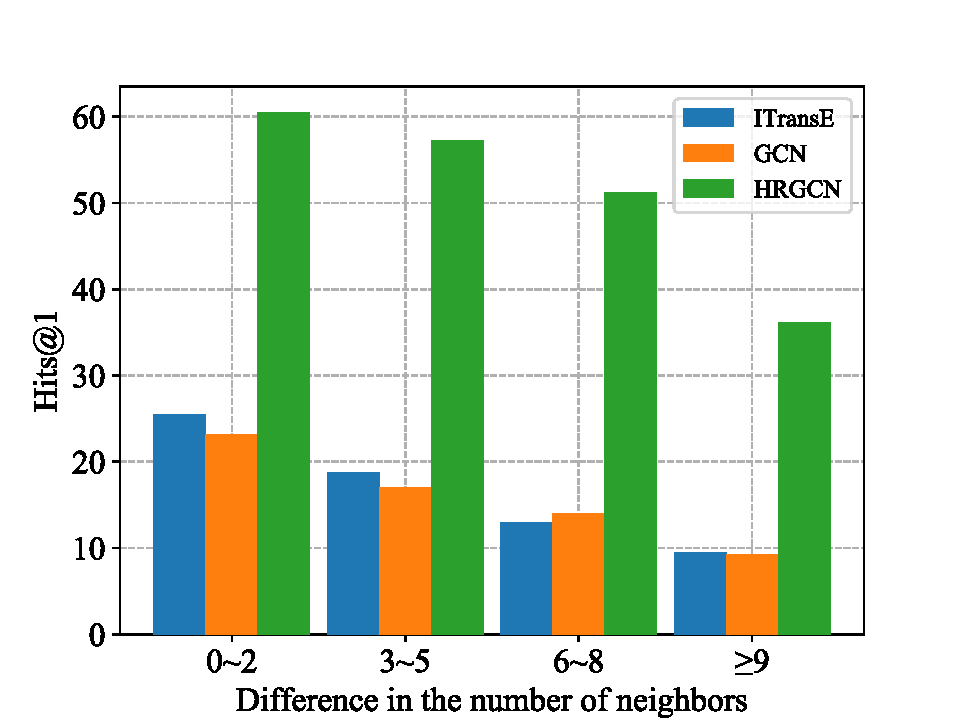
\includegraphics[width=1\linewidth]{figures/graph4.pdf}
	\caption{Hits@1 of ITransE$'$, \GCN and \HRGCN (SE+AE) on the four WBD subsets. 0$\sim$2 denotes the subset in which the number of neighbors differs from 0 to 2 for each entity pair, and similar for the remaining subsets.}
	\label{subset}
\end{figure}

Moreover, we randomly select several examples from WBD test set in Table~\ref{example},
%that our \HRGCN model can correctly align but ITransE$'$ fails in Table~\ref{example},
as well as their neighbor information, i.e., number of neighbors, number of values, number of potentially overlapped neighbors or values for each pair.
We can find that although some entities have dozens of neighbors in their own KGs, but their potentially overlapped neighbors are quite few, showing again that
%the number of similar neighbors of these entity pairs is no more than 6 which is very small compared to the number of their neighbors. This indicates that
the available clues for entity alignment are sparse,
 where ITransE$'$ fails to locate discriminative neighbors but \HRGCN (SE+AE) can still identify useful structure information from such limited clues.

We can also observe that attribute values play an important role in entity alignment.
For instance, in the entity pair about \textit{Hubei Province}, nearly half of the neighbors for each entity are values, and among all 5 similar neighbors, 3 of them are actually values,
which provide crucial supporting evidence for the final prediction. Unfortunately, ITransE$'$ does not utilize those information, thus is unable to collect sufficient evidence.

\begin{table}
	\centering
	\scriptsize
	\begin{tabular}{lcrcr}
		\toprule
		\multirow{2}{*}{\bf Aligned Entities} & \bf \#Neighbors & \bf \#Similar & \bf \#Values & \bf \#Similar \\
		&\bf  Wiki \& Baidu &\bf  Neighbors &\bf  Wiki \& Baidu &\bf  Values \\
		\midrule
		Deng Jiaxian & 10 \& 33 & 5 & \ 3 \& 11 & 2\\
		Hubei Province & 21 \& 50 & 5 & 10 \& 19 & 3\\
		European Union & 66 \& 35 & 6 & 18 \& 8\ \ \ & 2\\
		%Huazhong University of & \multirow{2}{*}{11 \& 32} & \multirow{2}{*}{4} & \multirow{2}{*}{8 \& 6} & \multirow{2}{*}{1}\\
		%Science and Technology & & & & \\
		%Huazhong University of Science and Technology & 11 \& 32 & 4 & 8 \& 6 & 1 \\
		Confucius & 10 \& 20 & 4 & 7 \& 3 & 2\\
		\bottomrule
	\end{tabular}
	\caption{The statistics of example entity pairs, which our \HRGCN(SE+AE) model correctly aligns but ITransE$'$ fails.}
	\label{example}
\end{table}


\cparagraph{Highway gates}
Adding more \HRGCN layers can help the center entities obtain information from neighbors that are multiple hops away. However, it might also introduce noisy information from the exponentially increasing neighbors, leading to significant decline in performance as shown in Figure~\ref{highway}, when no highway gates are used. We can observe that the performance of two-layered \RGCNs with highway gates improves upon one-layered \RGCN. Then by adding more layers the performance of highway \RGCNs decreased slowly, but much slower than \RGCNs without gates. This confirms that the highway gates effectively control the required balance of neighbor information transmission in \RGCNs.

In addition, from Table~\ref{f1}, we can see that the \GCN or \RGCN-based models with highway gates consistently achieve better performance than no-highway ones, indicating that highway gates can effectively improve the performance of both multi-layered \GCN and \RGCN models.
\begin{figure}
	\centering
	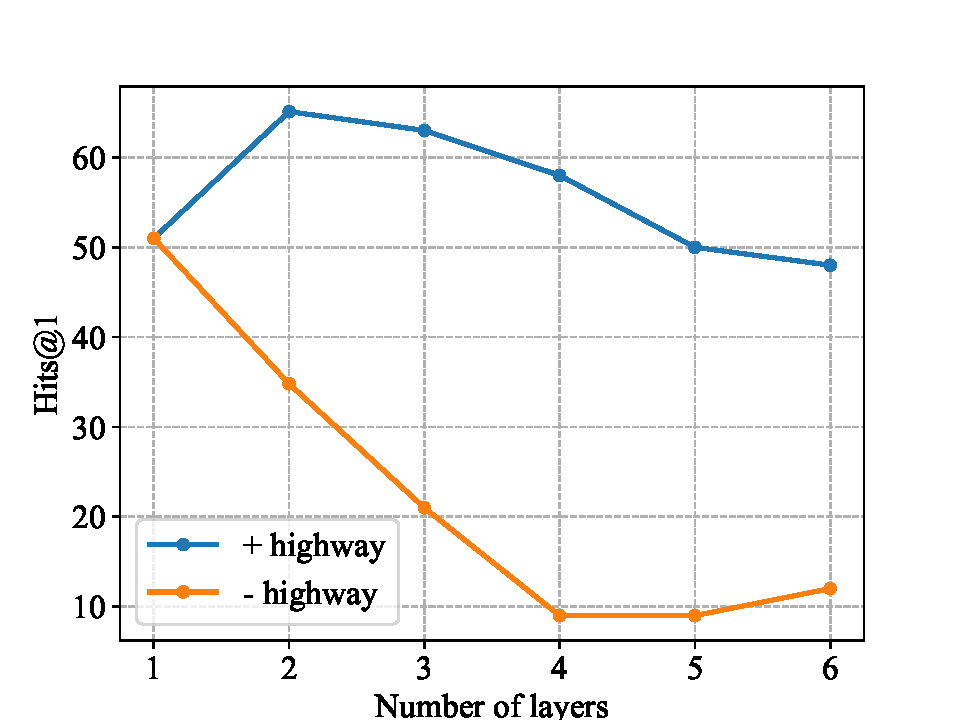
\includegraphics[width=1\linewidth]{figures/graph3.pdf}
	\caption{The effect of adding more \RGCN layers in terms of Hits@1 over the test set of WBD with and without the highway gates.}
	\label{highway}
\end{figure}
